\documentclass[openany]{tufte-book} % Use the tufte-book class which in turn uses the tufte-common class
\hypersetup{colorlinks} % Comment this line if you don't wish to have colored links
\usepackage{microtype} % Improves character and word spacing
\usepackage{booktabs} % Better horizontal rules in tables
\usepackage{tikz,tkz-graph,tkz-berge}
\usetikzlibrary{positioning}
\usepackage{verbatim, xcolor}
\usepackage{amsmath,amssymb}

\usetikzlibrary{arrows}
\usetikzlibrary{decorations.markings}
\newcommand{\boundellipse}[3]% center, xdim, ydim
{(#1) ellipse (#2 and #3)
}
\usepackage{graphicx} % Needed to insert images into the document
\graphicspath{{graphics/}} % Sets the default location of pictures
\setkeys{Gin}{width=\linewidth,totalheight=\textheight,keepaspectratio} % Improves figure scaling

\usepackage{fancyvrb} % Allows customization of verbatim environments
\fvset{fontsize=\normalsize} % The font size of all verbatim text can be changed here

\newcommand{\hangp}[1]{\makebox[0pt][r]{(}#1\makebox[0pt][l]{)}} % New command to create parentheses around text in tables which take up no horizontal space - this improves column spacing
\newcommand{\hangstar}{\makebox[0pt][l]{*}} % New command to create asterisks in tables which take up no horizontal space - this improves column spacing

\usepackage{xspace} % Used for printing a trailing space better than using a tilde (~) using the \xspace command

\newcommand{\monthyear}{\ifcase\month\or January\or February\or March\or April\or May\or June\or July\or August\or September\or October\or November\or December\fi\space\number\year} % A command to print the current month and year

\newcommand{\openepigraph}[2]{ % This block sets up a command for printing an epigraph with 2 arguments - the quote and the author
\begin{fullwidth}
\sffamily\large
\begin{doublespace}
\noindent\allcaps{#1}\\ % The quote
\noindent\allcaps{#2} % The author
\end{doublespace}
\end{fullwidth}
}

\newcommand{\blankpage}{\newpage\hbox{}\thispagestyle{empty}\newpage} % Command to insert a blank page

\usepackage{units} % Used for printing standard units

\newcommand{\hlred}[1]{\textcolor{Maroon}{#1}} % Print text in maroon
\newcommand{\hangleft}[1]{\makebox[0pt][r]{#1}} % Used for printing commands in the index, moves the slash left so the command name aligns with the rest of the text in the index 
\newcommand{\hairsp}{\hspace{1pt}} % Command to print a very short space
\newcommand{\ie}{\textit{i.\hairsp{}e.}\xspace} % Command to print i.e.
\newcommand{\eg}{\textit{e.\hairsp{}g.}\xspace} % Command to print e.g.
\newcommand{\na}{\quad--} % Used in tables for N/A cells
\newcommand{\measure}[3]{#1/#2$\times$\unit[#3]{pc}} % Typesets the font size, leading, and measure in the form of: 10/12x26 pc.
\newcommand{\tuftebs}{\symbol{'134}} % Command to print a backslash in tt type in OT1/T1

\providecommand{\XeLaTeX}{X\lower.5ex\hbox{\kern-0.15em\reflectbox{E}}\kern-0.1em\LaTeX}
\newcommand{\tXeLaTeX}{\XeLaTeX\index{XeLaTeX@\protect\XeLaTeX}} % Command to print the XeLaTeX logo while simultaneously adding the position to the index

\newcommand{\doccmdnoindex}[2][]{\texttt{\tuftebs#2}} % Command to print a command in texttt with a backslash of tt type without inserting the command into the index

\newcommand{\doccmddef}[2][]{\hlred{\texttt{\tuftebs#2}}\label{cmd:#2}\ifthenelse{\isempty{#1}} % Command to define a command in red and add it to the index
{ % If no package is specified, add the command to the index
\index{#2 command@\protect\hangleft{\texttt{\tuftebs}}\texttt{#2}}% Command name
}
{ % If a package is also specified as a second argument, add the command and package to the index
\index{#2 command@\protect\hangleft{\texttt{\tuftebs}}\texttt{#2} (\texttt{#1} package)}% Command name
\index{#1 package@\texttt{#1} package}\index{packages!#1@\texttt{#1}}% Package name
}}

\newcommand{\doccmd}[2][]{% Command to define a command and add it to the index
\texttt{\tuftebs#2}%
\ifthenelse{\isempty{#1}}% If no package is specified, add the command to the index
{%
\index{#2 command@\protect\hangleft{\texttt{\tuftebs}}\texttt{#2}}% Command name
}
{%
\index{#2 command@\protect\hangleft{\texttt{\tuftebs}}\texttt{#2} (\texttt{#1} package)}% Command name
\index{#1 package@\texttt{#1} package}\index{packages!#1@\texttt{#1}}% Package name
}}

% A bunch of new commands to print commands, arguments, environments, classes, etc within the text using the correct formatting
\newcommand{\docopt}[1]{\ensuremath{\langle}\textrm{\textit{#1}}\ensuremath{\rangle}}
\newcommand{\docarg}[1]{\textrm{\textit{#1}}}
\newenvironment{docspec}{\begin{quotation}\ttfamily\parskip0pt\parindent0pt\ignorespaces}{\end{quotation}}
\newcommand{\docenv}[1]{\texttt{#1}\index{#1 environment@\texttt{#1} environment}\index{environments!#1@\texttt{#1}}}
\newcommand{\docenvdef}[1]{\hlred{\texttt{#1}}\label{env:#1}\index{#1 environment@\texttt{#1} environment}\index{environments!#1@\texttt{#1}}}
\newcommand{\docpkg}[1]{\texttt{#1}\index{#1 package@\texttt{#1} package}\index{packages!#1@\texttt{#1}}}
\newcommand{\doccls}[1]{\texttt{#1}}
\newcommand{\docclsopt}[1]{\texttt{#1}\index{#1 class option@\texttt{#1} class option}\index{class options!#1@\texttt{#1}}}
\newcommand{\docclsoptdef}[1]{\hlred{\texttt{#1}}\label{clsopt:#1}\index{#1 class option@\texttt{#1} class option}\index{class options!#1@\texttt{#1}}}
\newcommand{\docmsg}[2]{\bigskip\begin{fullwidth}\noindent\ttfamily#1\end{fullwidth}\medskip\par\noindent#2}
\newcommand{\docfilehook}[2]{\texttt{#1}\index{file hooks!#2}\index{#1@\texttt{#1}}}
\newcommand{\doccounter}[1]{\texttt{#1}\index{#1 counter@\texttt{#1} counter}}

\usepackage{remreset}% to allow continuous numbering of figures/tables throughout the entire book

\makeatletter% since we're using commands with @ in their name
\@removefromreset{figure}{chapter}% don't reset figure numbering
\@removefromreset{table}{chapter}% don't reset figure numbering
\let\origappendix\appendix% save a copy of the original meaning of \appendix
\renewcommand{\appendix}{%
  \origappendix% do all the original \appendix stuff
  \titlecontents{chapter}%
    [0em] % distance from left margin
    {\vspace{1.5\baselineskip}\begin{fullwidth}\LARGE\rmfamily\itshape} % above (global formatting of entry)
    {\hspace*{0em}\appendixname~\thecontentslabel: } % before w/label (label = ``2'')
    {\hspace*{0em}} % before w/o label
    {\rmfamily\upshape\qquad\thecontentspage} % filler + page (leaders and page num)
    [\end{fullwidth}] % after
  \titleformat{\chapter}%
    [display]% shape
    {\relax\ifthenelse{\NOT\boolean{@tufte@symmetric}}{\begin{fullwidth}}{}}% format applied to label+text
    {\itshape\huge Appendix~\thechapter}% label
    {0pt}% horizontal separation between label and title body
    {\huge\rmfamily\itshape}% before the title body
    [\ifthenelse{\NOT\boolean{@tufte@symmetric}}{\end{fullwidth}}{}]% after the title body
  \setcounter{secnumdepth}{0}% ``number'' the appendices
  \renewcommand{\thefigure}{\@arabic\c@figure}% define \thefigure to use only the figure number (1), not A.1
  \renewcommand{\thetable}{\@arabic\c@table}%
  %
  % Add any other special appendix-related code here.
  %
}
\makeatother% restore the special meaning of @

\usepackage{makeidx} % Used to generate the index
\makeindex % Generate the index which is printed at the end of the document


\usepackage{amsmath, amsthm, amssymb}
\theoremstyle{plain}
\newtheorem{acknowledgement}{Acknowledgement}
\newtheorem{algorithm}{Algorithm}
\newtheorem{axiom}{Axiom}
\newtheorem{case}{Case}
\newtheorem{claim}{Claim}
\newtheorem{conclusion}{Conclusion}
\newtheorem{condition}{Condition}
\newtheorem{conjecture}{Conjecture}
\newtheorem{corollary}{Corollary}
\newtheorem{criterion}{Criterion}
\newtheorem{definition}{Definition}
\newtheorem{example}{Example}
\newtheorem{exercise}{Exercise}
\newtheorem{lemma}{Lemma}
\newtheorem{notation}{Notation}
\newtheorem{problem}{Problem}
\newtheorem{proposition}{Proposition}
\newtheorem{remark}{Remark}
\newtheorem{observation}{Observation}
\newtheorem{question}{Question}
\newtheorem{solution}{Solution}
\newtheorem{summary}{Summary}
\newtheorem{theorem}{Theorem}
\newtheorem*{HallsTheorem}{Hall's theorem}

\newcommand{\set}[1]{\left\{ #1 \right\}}
\newcommand{\setb}[3]{\left\{ #1 \in #2 : #3 \right\}}
\newcommand{\setbs}[2]{\left\{ #1 : #2 \right\}}
\newcommand{\card}[1]{\left|#1\right|}
\newcommand{\size}[1]{\left\Vert#1\right\Vert}
\newcommand{\ceil}[1]{\left\lceil#1\right\rceil}
\newcommand{\floor}[1]{\left\lfloor#1\right\rfloor}
\newcommand{\func}[3]{#1\colon #2 \rightarrow #3}
\newcommand{\funcinj}[3]{#1\colon #2 \hookrightarrow #3}
\newcommand{\funcsurj}[3]{#1\colon #2 \twoheadrightarrow #3}
\newcommand{\irange}[1]{\left[#1\right]}
\newcommand{\join}[2]{#1 \mbox{\hspace{2 pt}$\ast$\hspace{2 pt}} #2}
\newcommand{\djunion}[2]{#1 \mbox{\hspace{2 pt}$+$\hspace{2 pt}} #2}
\newcommand{\parens}[1]{\left( #1 \right)}
\newcommand{\brackets}[1]{\left[ #1 \right]}
\newcommand{\DefinedAs}{\mathrel{\mathop:}=}


\newcommand{\fancy}[1]{\mathcal{#1}}
%\newcommand{\C}[1]{\fancy{C}_{#1}}
\newcommand{\IN}{\mathbb{N}}
\newcommand{\IZ}{\mathbb{Z}}
\newcommand{\IR}{\mathbb{R}}
%\newcommand{\G}{\fancy{G}}
\newcommand{\CC}{\fancy{C}}
\newcommand{\D}{\fancy{D}}
\newcommand{\T}{\fancy{T}}
\newcommand{\B}{\fancy{B}}
\renewcommand{\L}{\fancy{L}}
\newcommand{\HH}{\fancy{H}}
\newcommand{\Q}{\fancy{Q}}
\newcommand{\Z}{\fancy{Z}}

\newcommand{\pot}{\operatorname{pot}}
\newcommand{\mic}{\operatorname{mic}}
\newcommand{\AT}{\operatorname{AT}}
\newcommand{\col}{\operatorname{col}}
\newcommand{\ch}{\operatorname{ch}}
\newcommand{\type}{\operatorname{type}}
\newcommand{\nonsep}{\bar{S}}

\usepackage{makeidx} % Used to generate the index
\makeindex % Generate the index which is printed at the end of the document
\title{Graph theory\\ for philosophy}
\author{brian rabern \& landon rabern}

\begin{document}
%\frontmatter
\cleardoublepage
\begin{titlepage} % Suppresses headers and footers on the title page

	
	\scshape % Use small caps for all text on the title page
	
	\vspace*{\baselineskip} % White space at the top of the page
	
	%------------------------------------------------
	%	Title
	%------------------------------------------------
	
	
	
	\vspace{0.75\baselineskip} % Whitespace above the title
	
	{\Huge \noindent \textcolor{darkgray}{GRAPH THEORY \\FOR PHILOSOPHY}\\} % Title
	
	\vspace{3\baselineskip} % Whitespace below the title
	

	
	{\LARGE  \textcolor{darkgray}{BRIAN RABERN}\\ \textcolor{darkgray}{LANDON RABERN} \\} % authors
	
	\vspace{5\baselineskip} % Whitespace 
	
	
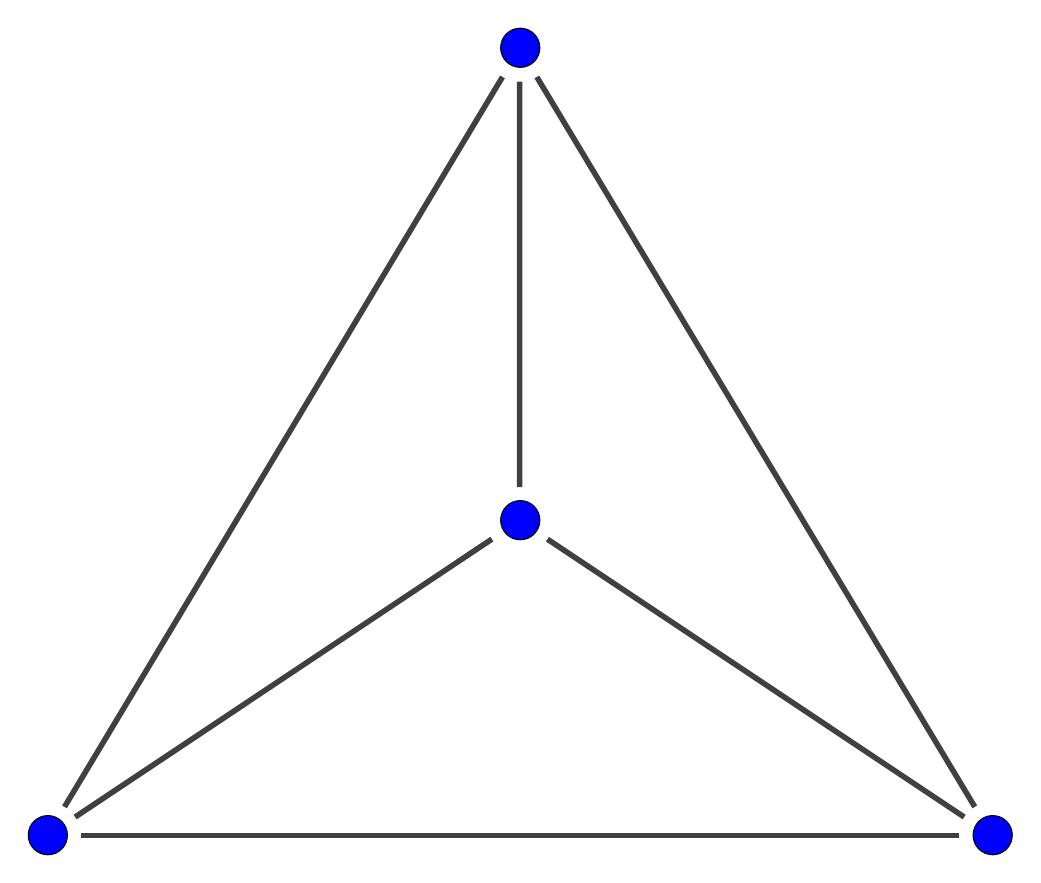
\begin{tikzpicture}[scale = 40]
\tikzstyle{VertexStyle} = []
\tikzstyle{EdgeStyle} = [line width=2pt, color=darkgray]
\tikzstyle{labeledStyle}=[shape = circle, minimum size = 6pt, inner sep = 5pt, outer sep = 5pt, draw]
\tikzstyle{unlabeledStyle}=[shape = circle, minimum size = 6pt, inner sep = 5pt, outer sep = 5pt, draw, fill]
\tikzstyle{5f873b39-9705-452a-a84b-434bd362e24f}=[shape = circle,minimum size = 6pt,inner sep = 5pt,outer sep = 5pt,draw,fill={rgb,255:red,0; green,0; blue,255}]
\tikzstyle{e8d2bc5d-1eaa-45b1-82c0-b5ad4369c905}=[shape = circle,minimum size = 6pt,inner sep = 5pt,outer sep = 5pt,draw,fill={rgb,255:red,0; green,0; blue,255}]
\tikzstyle{7cb4136b-f44e-4206-ba53-a1b49fb9c412}=[shape = circle,minimum size = 6pt,inner sep = 5pt,outer sep = 5pt,draw,fill={rgb,255:red,0; green,0; blue,255}]
\tikzstyle{5ca5c58d-8345-442a-887e-a790e621fc31}=[shape = circle,minimum size = 6pt,inner sep = 5pt,outer sep = 5pt,draw,fill={rgb,255:red,0; green,0; blue,255}]
\Vertex[style = 5f873b39-9705-452a-a84b-434bd362e24f, x = 0.600, y = 0.450, L = \tiny {}]{v0}
\Vertex[style = e8d2bc5d-1eaa-45b1-82c0-b5ad4369c905, x = 0.900, y = 0.450, L = \tiny {}]{v1}
\Vertex[style = 7cb4136b-f44e-4206-ba53-a1b49fb9c412, x = 0.750, y = 0.700, L = \tiny {}]{v2}
\Vertex[style = 5ca5c58d-8345-442a-887e-a790e621fc31, x = 0.750, y = 0.550, L = \tiny {}]{v3}
\Edge[label = \tiny {}, labelstyle={auto=right, fill=none}](v1)(v0)
\Edge[label = \tiny {}, labelstyle={auto=right, fill=none}](v2)(v0)
\Edge[label = \tiny {}, labelstyle={auto=right, fill=none}](v2)(v1)
\Edge[label = \tiny {}, labelstyle={auto=right, fill=none}](v3)(v2)
\Edge[label = \tiny {}, labelstyle={auto=right, fill=none}](v3)(v1)
\Edge[label = \tiny {}, labelstyle={auto=right, fill=none}](v3)(v0)
\end{tikzpicture}
\end{titlepage}



\tableofcontents

\mainmatter
\chapter{A brief history of graph theory}
A \emph{graph} is a collection of dots we call \emph{vertices} some of which are connected by curves we call \emph{edges}. 
The relative location of the dots and the shape of the curves are not relevant, we are only concerned with whether or not a given
pair of dots is connected by a curve.  Initially, we forbid edges from a vertex to itself and multiple edges between two vertices.
If $G$ is a graph, then $V(G)$ is its set of vertices and $E(G)$ its set of edges. 
We write $\card{G}$ for the number of vertices in $V(G)$ and $\size{G}$ for the number of edges in $E(G)$.
Two vertices
are \emph{adjacent}  if they are connected by an edge.  The set
of vertices to which $v$ is adjacent is its \emph{neighborhood}, written $N(v)$. 
For the size of $v$'s neighborhood $\card{N(v)}$, we write $d(v)$ and call this the \emph{degree} of $v$.
We write $E(v)$ for the set of edges containing $v$, these are the edges \emph{incident} to $v$.

We use the shorthand $\irange{k} \DefinedAs \set{1,2,\ldots, k}$. A \emph{path} in $G$ is a sequence of different vertices $x_1, x_2, \ldots, x_r$ such that $x_i$ is 
adjacent to $x_{i+1}$ for all $i \in \irange{r-1}$.  We say
this is a path from $x_1$ to $x_r$.
If $x_r$ is adjacent to $x_1$ as well, then we have a \emph{cycle}.  A graph $G$ is \emph{connected} if for all $x,y \in V(G)$, there is a path from $x$ to $y$.
Figure \ref{fig:SmallGraphs} shows all the connected graphs with at most five vertices.

\begin{marginfigure}
		\includegraphics[width=0.5in]{graphs/all/0.pdf}
		\includegraphics[width=0.5in]{graphs/all/1.pdf}
		\includegraphics[width=0.5in]{graphs/all/011.pdf}
		\includegraphics[width=0.5in]{graphs/all/111.pdf}
		\includegraphics[width=0.5in]{graphs/all/001011.pdf}
		\includegraphics[width=0.5in]{graphs/all/011010.pdf}
		\includegraphics[width=0.5in]{graphs/all/011011.pdf}
		\includegraphics[width=0.5in]{graphs/all/011110.pdf}
		\includegraphics[width=0.5in]{graphs/all/011111.pdf}
		\includegraphics[width=0.5in]{graphs/all/111111.pdf}
		\includegraphics[width=0.5in]{graphs/all/0001001011.pdf}
		\includegraphics[width=0.5in]{graphs/all/0011001010.pdf}
		\includegraphics[width=0.5in]{graphs/all/0011001011.pdf}
		\includegraphics[width=0.5in]{graphs/all/0011010011.pdf}
		\includegraphics[width=0.5in]{graphs/all/0011011010.pdf}
		\includegraphics[width=0.5in]{graphs/all/0011011011.pdf}
		\includegraphics[width=0.5in]{graphs/all/0011011110.pdf}
		\includegraphics[width=0.5in]{graphs/all/0011011111.pdf}
		\includegraphics[width=0.5in]{graphs/all/0101011000.pdf}
		\includegraphics[width=0.5in]{graphs/all/0101011010.pdf}
		\includegraphics[width=0.5in]{graphs/all/0101011011.pdf}
		\includegraphics[width=0.5in]{graphs/all/0110011010.pdf}
		\includegraphics[width=0.5in]{graphs/all/0111001110.pdf}
		\includegraphics[width=0.5in]{graphs/all/0111001111.pdf}
		\includegraphics[width=0.5in]{graphs/all/0111011010.pdf}
		\includegraphics[width=0.5in]{graphs/all/0111011011.pdf}
		\includegraphics[width=0.5in]{graphs/all/0111011111.pdf}
		\includegraphics[width=0.5in]{graphs/all/0111111010.pdf}
		\includegraphics[width=0.5in]{graphs/all/0111111011.pdf}
		\includegraphics[width=0.5in]{graphs/all/0111111111.pdf}
		\includegraphics[width=0.5in]{graphs/all/1111111111.pdf}
		\caption{The connected graphs with at most five vertices.}
		\label{fig:SmallGraphs}
\end{marginfigure}

\chapter{The basics of graph theory}

\backmatter
\appendix
\printindex
\end{document}